% Introduce the problem, motivation, and relevant background.
% Cite prior work using \cite{key} — entries go in references.bib.

% Subsection 1: Atalla top-level
% Systolic Array
% Memory subsystem
% Vector core
% Scheduler
\subsection{Atalla Top-Level Architecture}

At the heart of the architecture is a 32x32 systolic array of PEs operating under a weight-stationary dataflow. In this regime, filter weights are latched whithin each PE across multiple input activations, maximizing weight reuse and minimizing the energy cost of repeated memory fetches: the dominant source of power dissipation in matrix-intensive workloads \cite{efficientprocessingofdnn, sysarrfinalreport}.

Surrounding this compute fabric is a 2 MB software-controlled Scratchpad memory that replaces conventional hardware-managed caches with explicit, programmer-directed data movement. A tile-descriptor based direct memory acces (DMA) engine orchestrates bulk transfers between off-chip DRAM and the Scratchpad, while a bank-swizzling scheme permutes address mapping across memory banks to eliminate bank conflicts during wide vector accesses characteristic of GEMM tiling \cite{scpadfinalreport}.

Interfacing between the Scratchpad and the systolic array is a 32-wide Vector Core, a datapath responsible for managing data-level parallelism (DLP) accross the full width of the array. The Vector Core communicates with the systolic array through the Global Systolic Array Unit (GSAU), which coordinates activation feeding, weight loading and result extraction; and it communicates with the Scratchpad through the Vector Load Store (VLS) unit (or VLSU), sending reads and write requests \cite{vcfinalreport}.

A 4-wide Very Long Instruction Word (VLIW) scheduler orchestrates all functional units (FUs) by issuing instruction bundles each cycle and managing inter-bundle data dependencies statically \cite{schedulerfinalreport}. By delegating the complexity of parallelism detection from hardware to the compiler, the architecture significantly simplifies the control logic and reduces power overhead compared to superscalar designs \cite{simplevliw}.

% Subsection 2: Custom ISA
% What is our ISA
% Why do we use it, instead of RISCV + extensions
% Why this is a barrier from using established simulators
\subsection{Custom Instruction Set Architecture Rationale and Simulation Challenges}

\begin{figure}
    \centering
    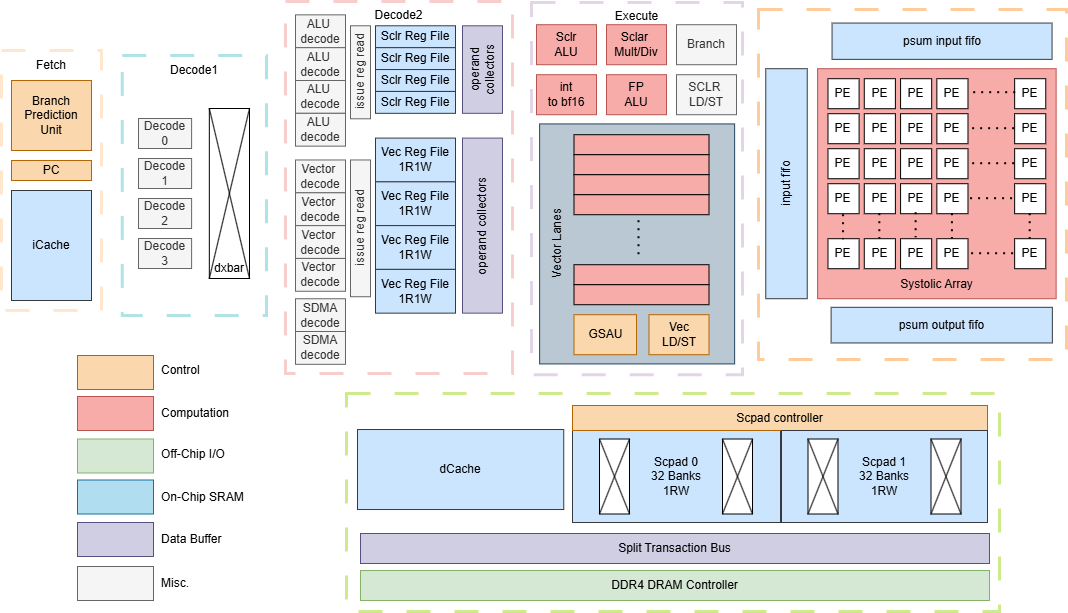
\includegraphics[width=1\linewidth]{figures/toplevelatalla-new.drawio.png}
    \caption{Atalla Ax01 Top-Level}
    \label{fig:toplevelatalla}
\end{figure}

Atalla utilizes a custom 40-bit Instruction Set Architecture (ISA) specifically optimized for tile-centric computing kernels. The ISA incorporates specialized instructions such as \texttt{gemm.vv} for initiating systolic array computations and \texttt{sdma} for orchestrating Scratchpad tile transfers \cite{sysarrfinalreport}. The design eliminates translation overhead and complex decode stades inherent in general-purpose architectures by mapping instructions directly to microarchitectural resources \cite{scpadfinalreport}. Standard alternatives like RISC-V Vector (RVV) introduce significant hardware bloat for domain-specific workloads by including support for Select Element Width (SEW), Extended Effective Width (EEW) and Length Multiplier (LMUL). These mandatory provisions require additional control logic and silicon area to support generality that is not exercised in an characterized AI accelerator  \cite{vcfinalreport, riscv, rvv}. A GEMM-native ISA allows the instruction encoding budget to be focused on high-throughput operations, resulting in a denser instruction stream and reduced decoder complexity \cite{sysarrfinalreport}.

In contrast, Atalla-Sim functions as a bespoke, functional validation framework by simulating Atalla’s Scratchpad traffic, vector datapath and systolic-array execution directly, bypassing the rigid front-end assumptions and legacy maintenance burden of general-purpose ISA simulators \cite{simplevliw}. Because it is specialized to handle the accelerator’s packetized, tile-oriented execution model, which requires modeling bonded "instruction lines" rather than the independent instruction tokens found in conventional superscalar engines, it can be adapted rapidly as the ISA and microarchitecture evolve \cite{casvliw}. This agility allows the simulator to serve as a critical tool for validating architectural intent and functional correctness against the hardware specification before the RTL is finalized. The cycle-accurate software environment complements rather than replaces RTL verification, providing a strong foundation for pre-silicon studies while acknowledging that RTL design remains a resource-intensive "mammoth task" \cite{unifiedmethpresiverif}.

As a result, an existing simulator cannot be used off the shelf to execute Atalla programs. Supporting the ISA would require implementing a new decoder for the 40-bit instruction format, defining the semantics of custom operations, and modeling accelerator-specific structures such as the scratchpad and systolic-array control path. These additions are substantial enough that the simulator would effectively need to be extended into a custom architectural model. For this reason, a purpose-built simulator is a more practical vehicle for functional validation of the Atalla ISA and its software stack.

% Subsection 3: VLIW
% What is VLIW
% Why is Atalla VLIW
% Previous work on VLIW simulation
% Why is it not possible on current simulators
\subsection{Simulating a Very Long Instruction Word Architecture}
The deterministic regularity of many dense DNN kernels creates a requirement for high levels of Instruction-Level Parallelism (ILP) \cite{scpadfinalreport, casvliw}. In these specific workloads, a sufficiently capable compiler can extract this parallelism statically, rendering the extensive dynamic scheduling hardware found in stock superscalar designs, such as large reservation stations and reorder buffers, unnecessary or of poor value \cite{vliw}.

To exploit this parallelism while minimizing hardware overhead, the Atalla architecture utilizes a Very Long Instruction Word (VLIW) model \cite{schedulerfinalreport}. VLIW shifts the tradeoff between ILP and hardware complexity by relocating the burden of parallelism detection from runtime hardware to the static compiler. Rather than employing complex dynamic scheduling logic, a VLIW processor exposes multiple functional unit slots within a single long instruction word, or instruction packet. The compiler analyzes data dependencies at compile time and packs independent operations into these slots, aiming to achieve high throughput with simplified control logic and reduced power overhead \cite{vliw}.

However, accurately simulating this VLIW mode reveals that stock superscalar CPU models in ecosystems like gem5 or SimpleScalar are often awkward and heavier-weight for this specific use case \cite{casvliw, simplevliw}. While Atalla-Sim draws structural inspiration from gem5’s modular class hierarchy, it avoids the overhead of the runtime dependency tracking and speculative execution engines that characterize the standard models in those frameworks \cite{casvliw, gem5}.

Atalla-Sim addresses these challenges by mirroring Atalla’s packetized execution model directly. The simulator groups instructions into VLIW packets which are then split into per-unit issue paths inside the Vector Core, specifically for the GSAU, the VLS, and the vector datapath, and bridged outward to the rest of the system as needed. This architecture correctly models the vector lanes as being downstream of the datapath issue path. This modeling approach accounts for structural hazards, such as functional unit slot limits and per-unit acceptance, which may cause packet contents to remain partially unissued across cycles. This modeling approach accounts for structural hazards, such as functional unit slot limits and per-unit acceptance, which may cause packet contents to remain partially unissued across cycles \cite{casvliw, unifiedmethpresiverif}.